\style{mq}
%   Titre de la sous sections
\section{Robot \mq et capteur de distance}

\subsection{Description}

\subsubsection{Objectif}

\begin{formule}
Le but de cette séquence est d’\textbf{utiliser} et d'\textbf{étalonner} le capteur de distance ultrasonique du robot \mq. Ce capteur sera utilisé en tant que télémètre.

Après un étalonnage utilisant un modèle linéaire, nous proposons de programmer le robot afin qu'il  s’arrête à une distance précise d’un obstacle.
\end{formule}


\subsubsection{Intérêt}


%liste d'arguments
\begin{description}
    \item [Capteur piézoélectrique] La mise en œuvre du détecteur permet d’utiliser un capteur piézoélectrique de façon concrète.
    \item [Propagation du son dans un milieu] Une explication théorique du fonctionnement du capteur permet de parler de la célérité du son dans l’air et de la notion d’ultrason.
    \item [Régression linéaire] L’étalonnage permet de mettre en application sur un cas concret la régression linéaire.
    \item [Mouvement du robot] La dernière partie permet de relier mouvement et détection, avec une automatisation basique. 
\end{description}


\subsubsection{Matériel}
\begin{itemize}
    \item 1 $\times$ \matosMb
    \item 1 $\times$ \matosMq (et son capteur intégré de distance ultrasonore)
    \item 1 $\times$ tableau magnétique
    \item 1 $\times$ règle graduée d'un mètre
    \item 1 $\times$ accès Internet :
    
    \begin{itemize}
        \item[$\bullet$] 1 $\times$ accès Internet : IDE programmation par bloc \url{http://makecode.microbit.org/}
        \item[$\bullet$] 1 $\times$ accès en ligne à l'extension pour la programmation par bloc du robot \mq :\\ \url{https://github.com/DFRobot/pxt-maqueen}
    \end{itemize}
    
\end{itemize}


\newpage
\subsubsection{Remarques}

\begin{wrapfigure}[9]{r}{5cm}
    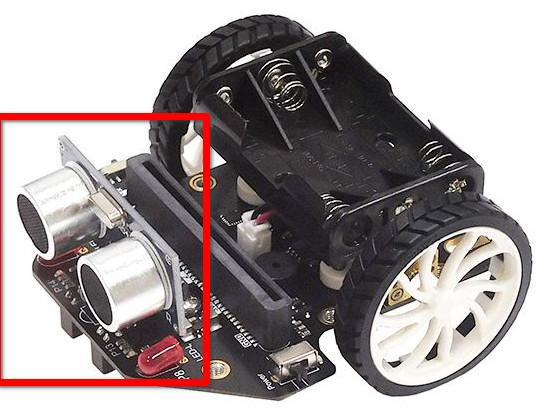
\includegraphics[width=\linewidth]
    {res/maqueen-fiche1-01.jpg}
\end{wrapfigure}

Le robot \mq est un robot pilotable à l’aide d’une carte \mb.\\
Ce dernier est équipé de 2 roues motorisées, d’un buzzer, de 2 leds rouges de signalements, de 4 leds Neopixel, de 2 capteurs de lignes, d’un capteur de télécommande infrarouge et d’un \textbf{capteur de distance à ultrason}. C’est ce dernier capteur que nous allons utiliser, ainsi que les moteurs. 


Le détecteur envoie une pulsation sonore de fréquence $40 kHz$ et mesure le temps que met l'onde pour faire l’aller-retour après réflexion sur un obstacle. Ce temps permet ainsi d’estimer une distance en reliant temps, célérité de l’onde et distance par la relation : $d = \frac{c \times t}{2}$ avec la distance $d$ en m, la célérité $c$ du son dans l’air en m/s et $t$ le temps en s.

Pour chaque robot, un \textbf{étalonnage} est obligatoire à chaque séance car :
\begin{itemize}
    \item la célérité dépend de la \textbf{température}
    \item l’\textbf{horloge interne} des \mb n’est pas très précises.
\end{itemize}~\\


\begin{methode}
\textbf{Installation de la bibliothèque \mq pour Makecode}


    
\begin{enumerate}
    \item Dans l’éditeur Makecode de Viens Coder, cliquer sur le bouton « Extension ».\\
    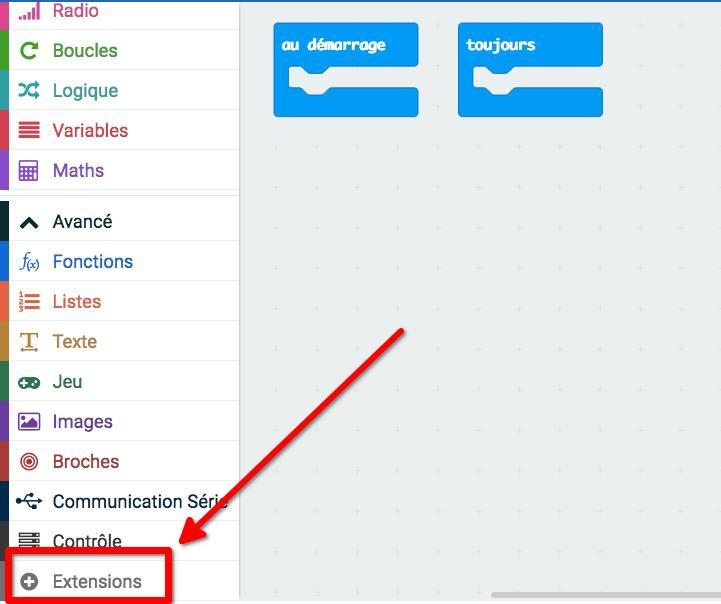
\includegraphics[width=0.5\linewidth]
    {res/maqueen-fiche1-02.jpg}
    
    \item Dans l’interface de recherche, entrer l’adresse suivante : \url{https://github.com/DFRobot/pxt-maqueen}\\
    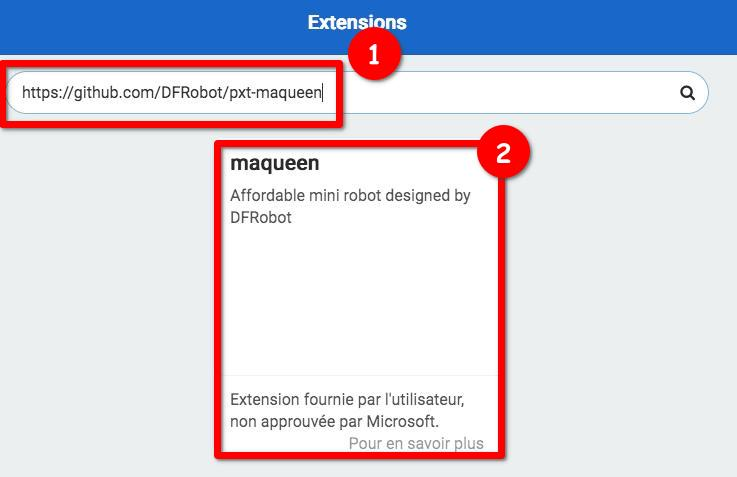
\includegraphics[width=0.5\linewidth]
    {res/maqueen-fiche1-03.jpg}
    
    \item Cliquer sur \textit{\mq} et une nouvelle famille de blocs apparait.\\
    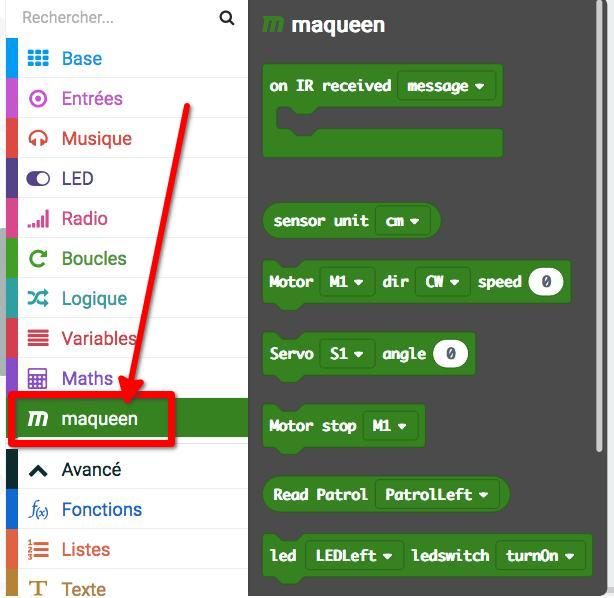
\includegraphics[width=0.5\linewidth]
    {res/maqueen-fiche1-04.jpg}
    
    \item Le bloc \textit{sensor unit} permet de mesurer la distance, \textit{Motor} à faire tourner les moteurs (\textbf{M1} gauche, \textbf{M2} droit) et \textit{Motor stop} à les arrêter.
\end{enumerate}
\end{methode}



\newpage


\subsection{Niveau initiation - Utilisation du capteur de distance à ultrasons}

\subsubsection{Activité élève}

\cartouche
{0,5 h}         %durée
{2de}           %public
{}        %maths
{}     %sciences
{}       %algo



\begin{wrapfigure}[4]{r}{3cm}
    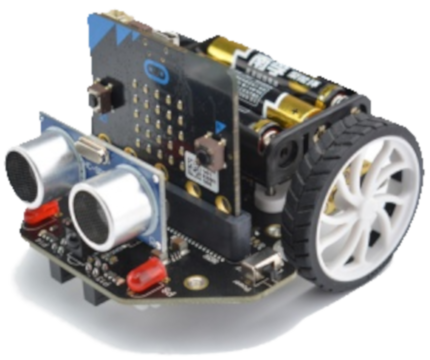
\includegraphics[width=\linewidth]{res/mini-maqueen.png}
\end{wrapfigure}


\begin{eleve}
    Première programme avec le robot \mq.
    
    \texttt{\textsc{Ta Mission} : Sauras-tu utiliser le programme ci-dessous pour \textbf{programmer} ton robot \mq?}
    
%   ajout d'une image
    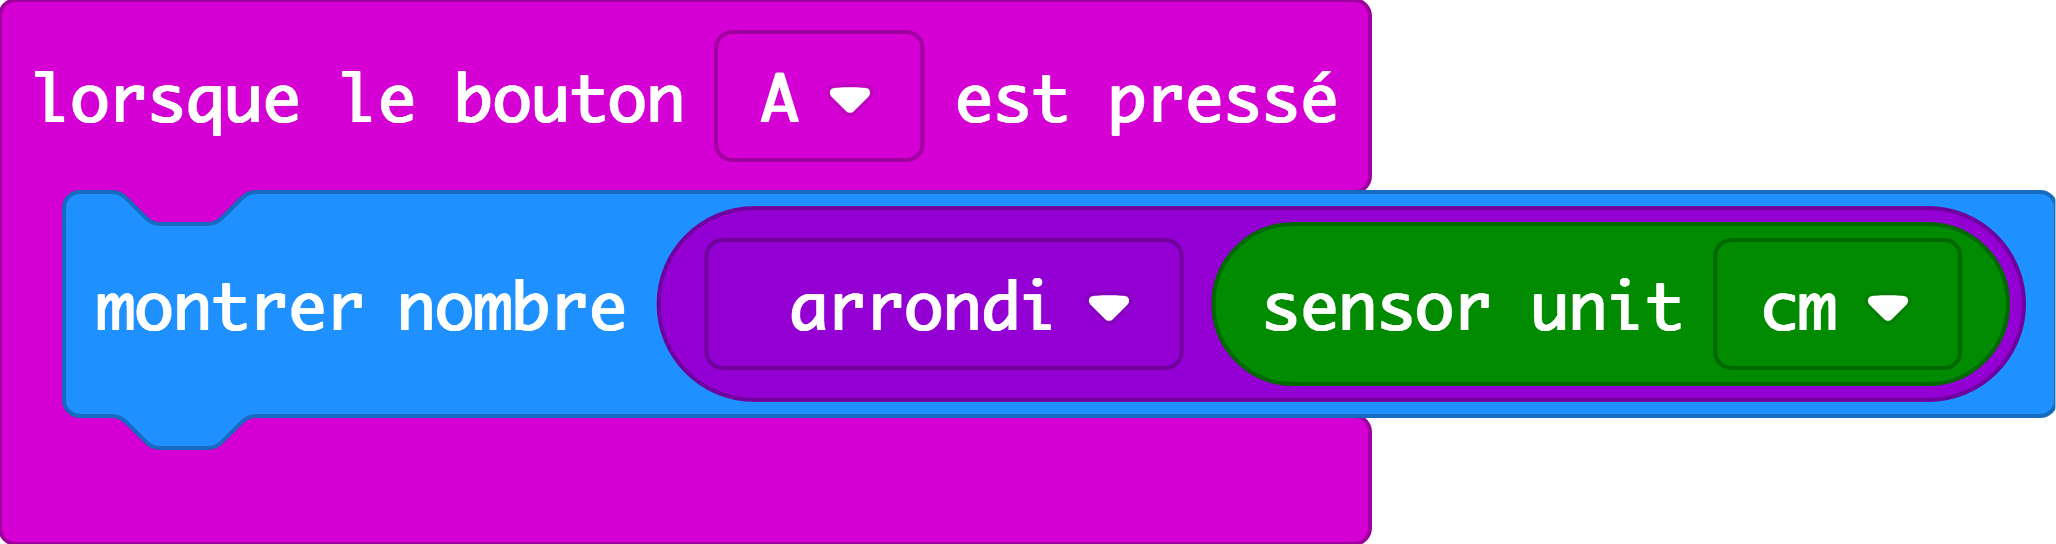
\includegraphics[width=0.5\linewidth]{res/maqueen-fiche1-10.png}
\end{eleve}



\subsubsection{Notes pour l'enseignant}

%
%   méthode et remarque
%
\begin{methode}
Proposition de résolution :
\begin{itemize}
    \item Télécharger le programme puis le téléverser sur la carte \mb.
    \item Insérer la carte dans le robot \mq.
    \item Tester le programme en mesurant la distance (bouton A) à divers objets et chercher les limites du détecteur (angle de visée, objet non plat…)
\end{itemize} 
\end{methode}


\begin{remarque}
    Nous rappelons qu'il est indispensable d'installer l'extension \mq sur l'interface Makecode  (\url{https://github.com/DFRobot/pxt-maqueen})
\end{remarque}






\newpage


\subsection{Niveau intermédiaire - Étalonnage du capteur}

\subsubsection{Activité élève}

\cartouche
{1,5 h}         %durée
{2de, 1ère, Term}           %public
{nuage de points, régression linéaire}        %maths
{}     %sciences
{}       %algo



\begin{wrapfigure}[4]{r}{3cm}
    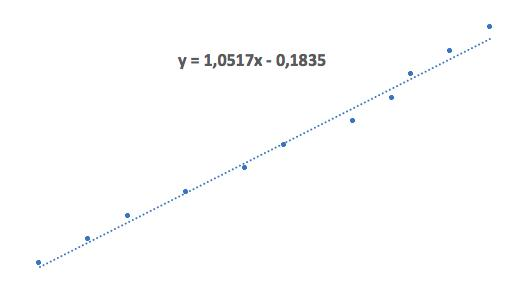
\includegraphics[width=\linewidth]{res/maqueen-fiche1-20.jpg}
\end{wrapfigure}


\begin{eleve}

    Le capteur du robot \mq est très précis, mais malheureusement il donne souvent des valeurs faussées à cause de la chaleur et de la carte \mb.
    
    Pour corriger cela, il est indispensable de l'\textbf{étalonner}.
    
   
    \texttt{\textsc{Ta Mission} : Nous avons besoin de toi pour étalonner le robot \mq de la classe.
    }~\\
    
    Si tu le désires, tu peux utiliser une règle, un obstacle (comme un tableau magnétique) et t'inspirer des deux indices ci-dessous\ldots
    
%   ajout d'une image
    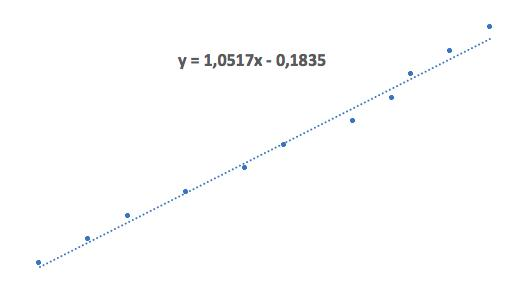
\includegraphics[scale=0.6]{res/maqueen-fiche1-20.jpg}
    \hfill
    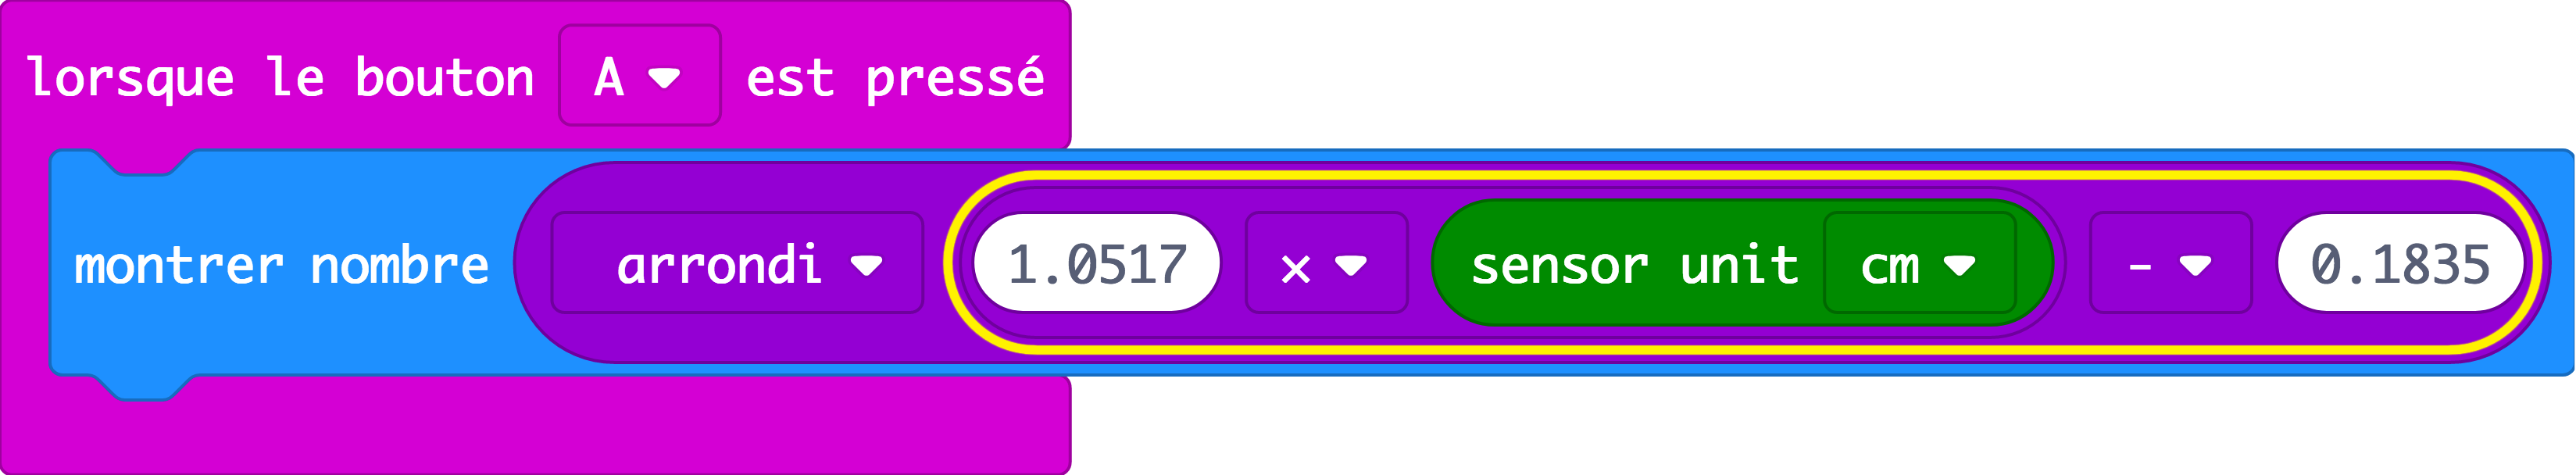
\includegraphics[width=0.45\linewidth]{res/maqueen-fiche1-21.png}
\end{eleve}



\subsubsection{Notes pour l'enseignant}

\begin{methode}~\\

Proposition de méthode de résolution :

\begin{enumerate}
    \item Placer le robot à 10 cm, 15 cm,20 cm \ldots 100 cm d’un tableau de mécanique faisant obstacle.
    \item Relever avec le capteur du robot les distances.
    \item Renouveler l’opération pour chaque distance.
    \item Dans un tableur, tracer la distance réelle en fonction de la distance mesurée par le capteur.
    \item Modéliser le nuage de points par une régression linéaire.
    \item Avec les blocs \textit{Maths}, corriger le programme original pour afficher désormais une distance plus proche de la distance réelle prenant en compte la régression.
\end{enumerate}
\end{methode}




\newpage


\subsection{Niveau expert - Robot autonome}

\subsubsection{Activité élève}

\cartouche
{1 h}           %durée
{1ère, Term}    %public
{}              %maths
{}              %sciences
{}              %algo



\begin{wrapfigure}[4]{r}{3cm}
    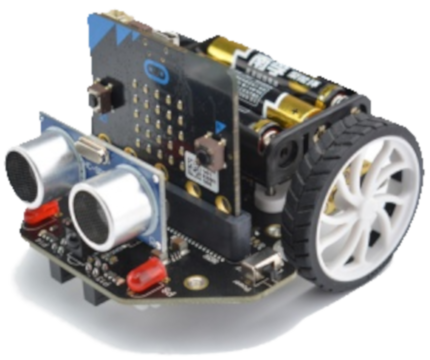
\includegraphics[width=\linewidth]{res/mini-maqueen.png}
\end{wrapfigure}


\begin{eleve}

    \texttt{\textsc{Ta Mission} : Programme le robot \mq pour qu'il avance quand on appuie sur le bouton A puis s'arrête à 20 cm d'un obstacle.
    }
\end{eleve}



\subsubsection{Notes pour l'enseignant}

\begin{minipage}[t]{0.5\linewidth}
    \begin{methode}~\\
    Proposition de résolution :
    
    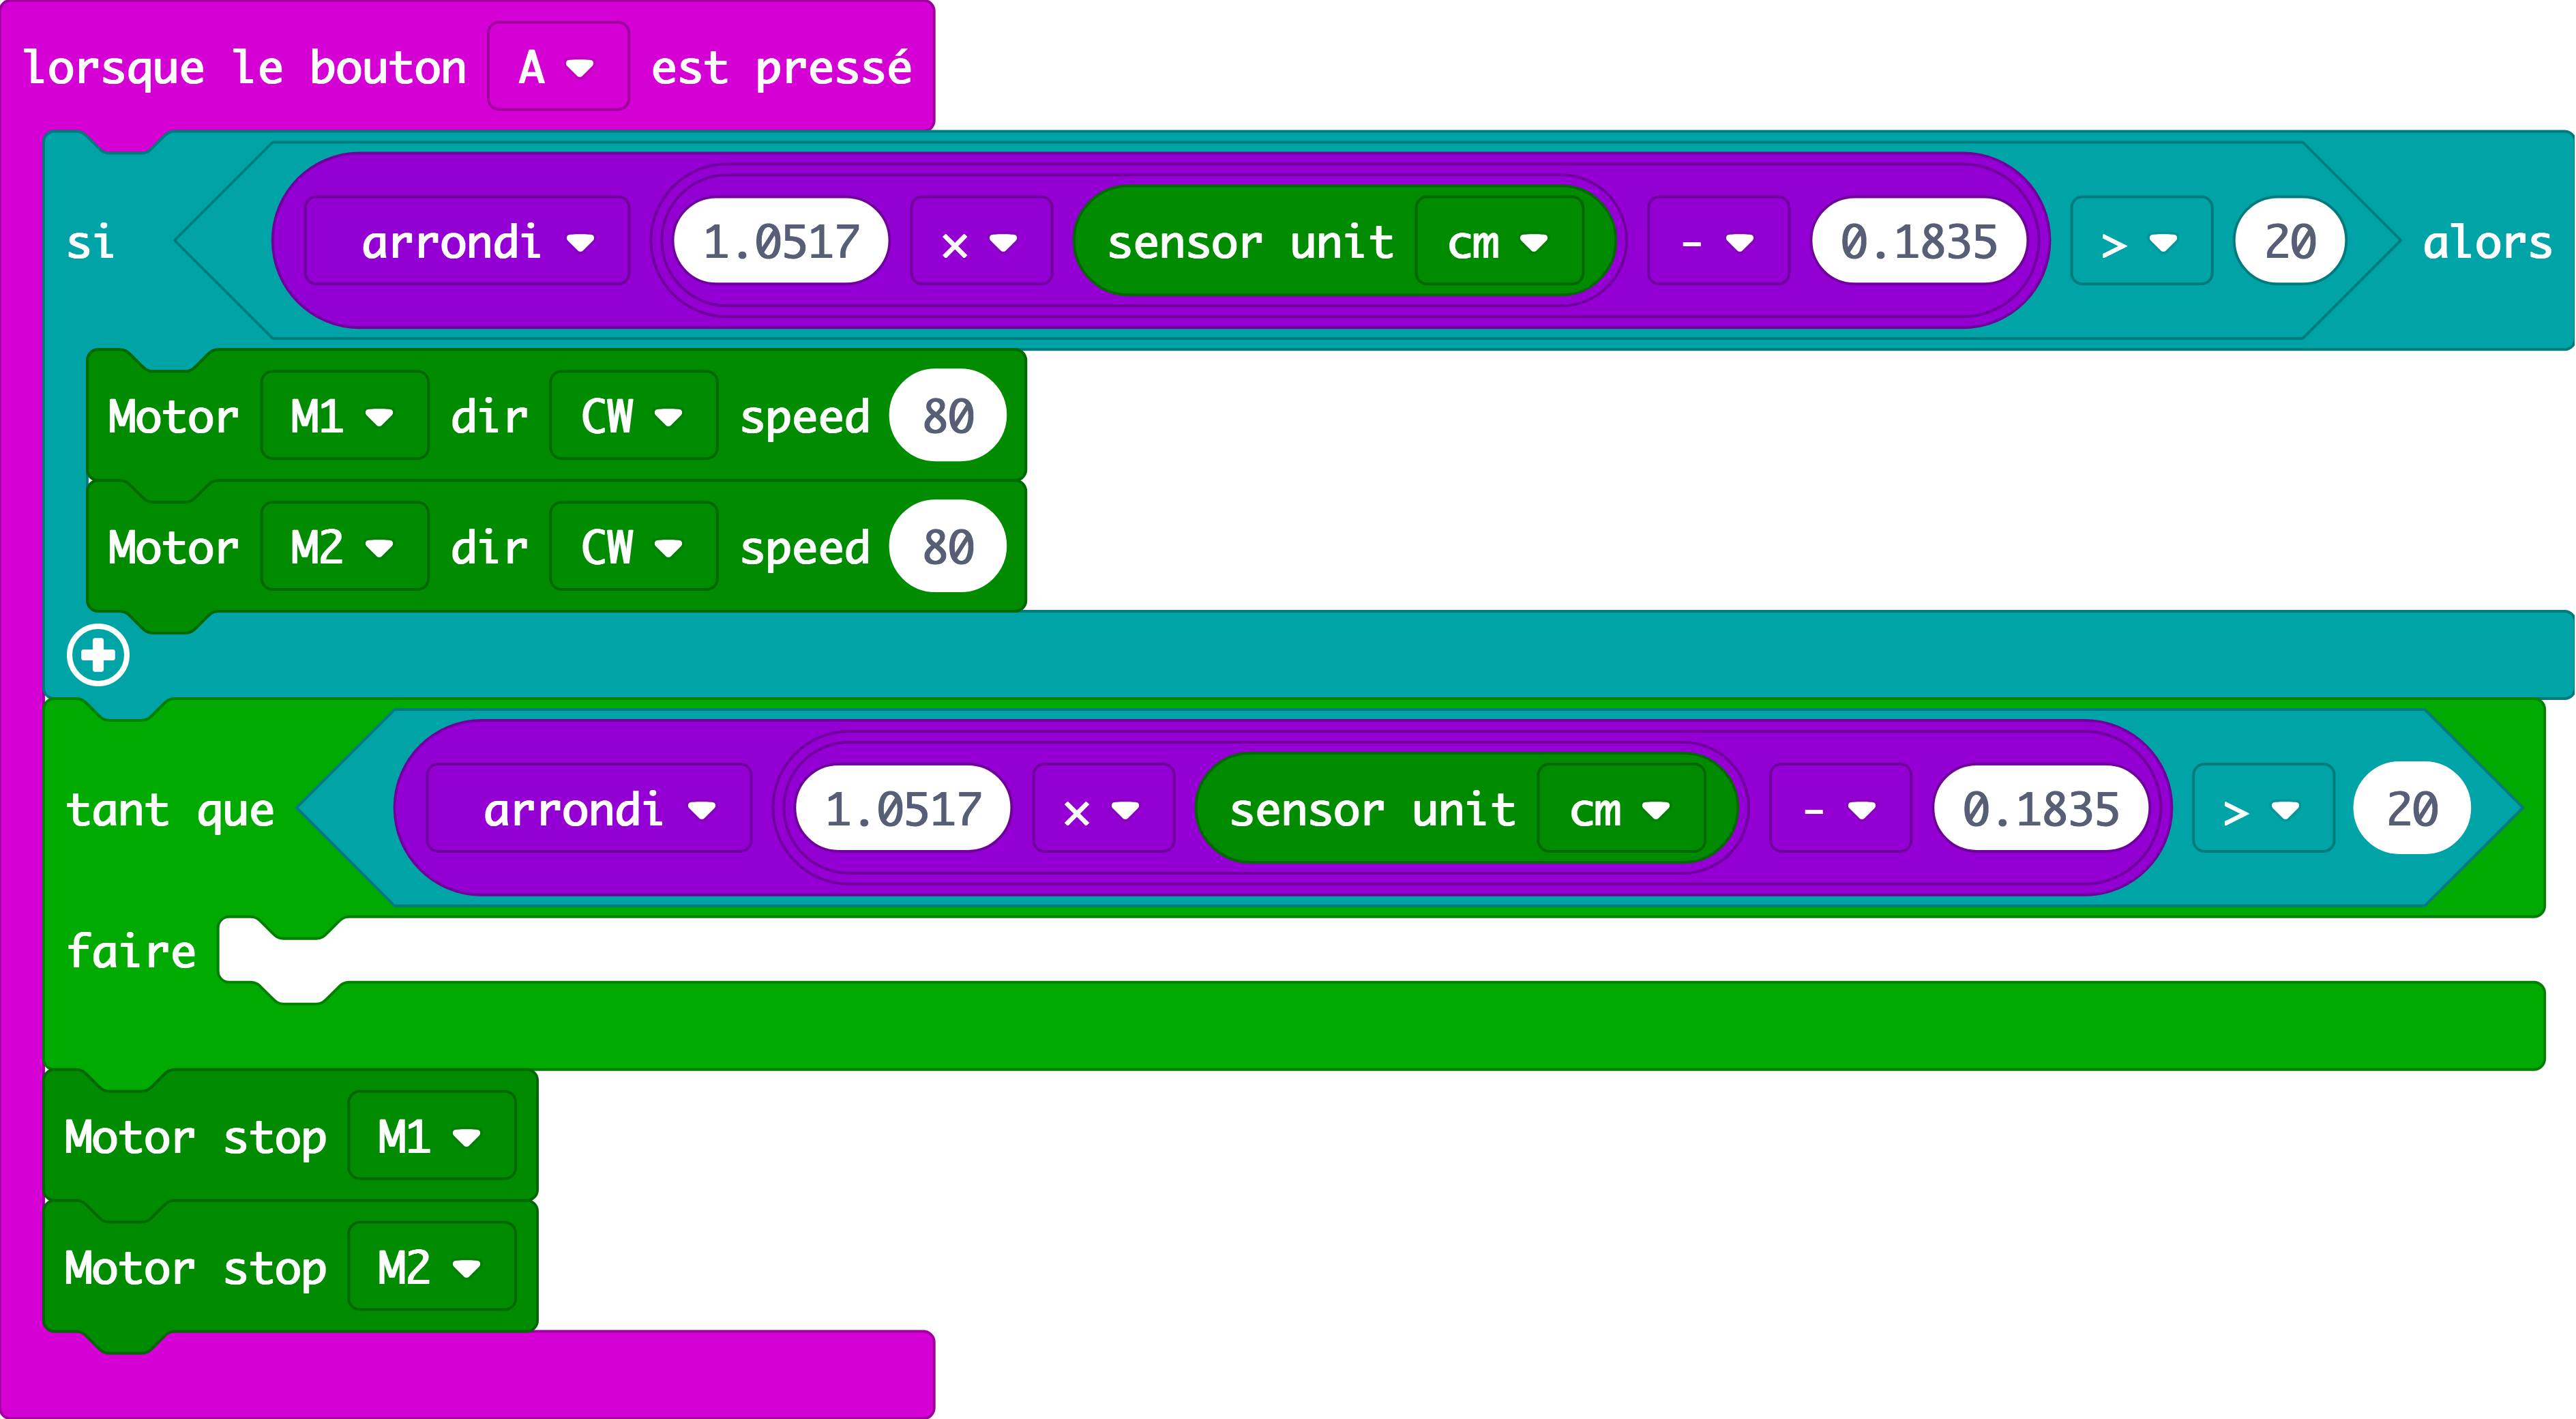
\includegraphics[width=\linewidth]
    {res/maqueen-fiche1-30.png}
    
    \end{methode}
\end{minipage}
\hfill
\begin{minipage}[t]{0.5\linewidth}
    \begin{remarque}~\\
    Les élèves peuvent aussi programmer un \textbf{radar de recul} en utilisant aussi le \textbf{haut-parleur} du robot \mq.
    
    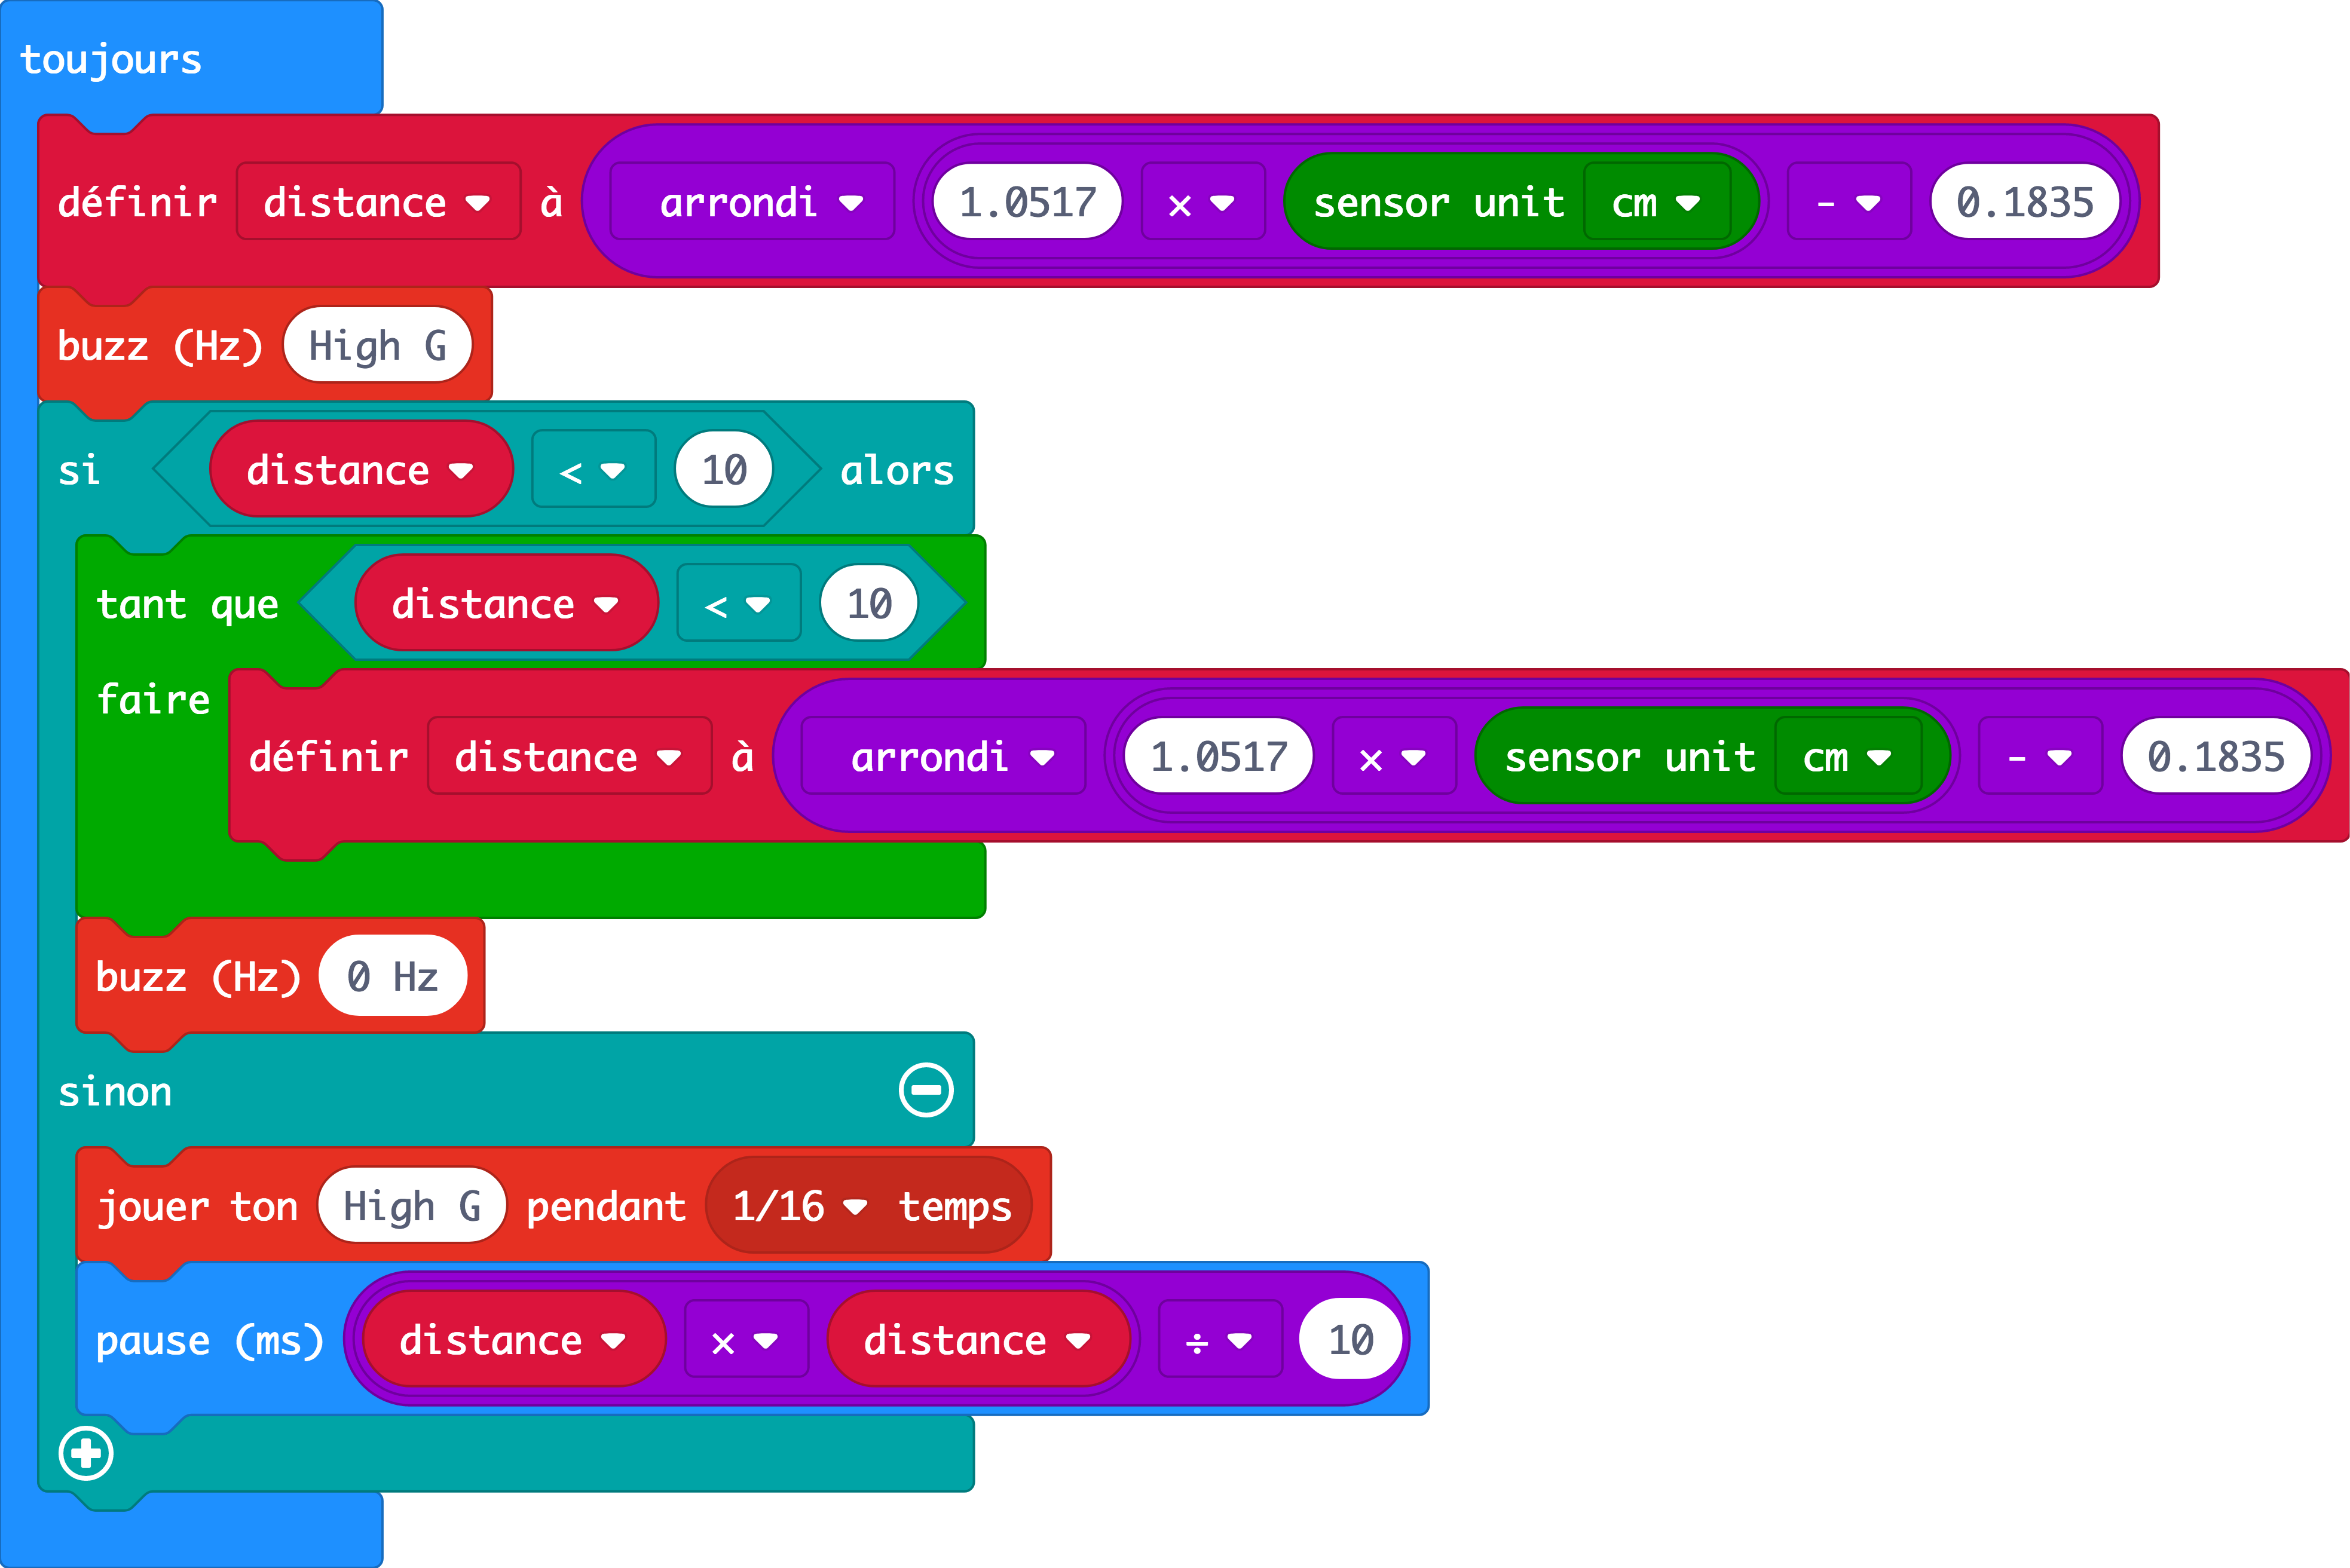
\includegraphics[width=\linewidth]
    {res/maqueen-fiche1-31.png}
    
    
    \end{remarque}
\end{minipage}